\documentclass{article}

\usepackage{fullpage}
\usepackage{color}
\usepackage{amsmath}
\usepackage{url}
\usepackage{verbatim}
\usepackage{graphicx}
\usepackage{parskip}
\usepackage{amssymb}
\usepackage{nicefrac}
\usepackage{listings} % For displaying code
\usepackage{algorithm2e} % pseudo-code

% Answers
\def\ans#1{\par\gre{Answer: #1}}

% Colors
\definecolor{blu}{rgb}{0,0,1}
\def\blu#1{{\color{blu}#1}}
\definecolor{gre}{rgb}{0,.5,0}
\def\gre#1{{\color{gre}#1}}
\definecolor{red}{rgb}{1,0,0}
\def\red#1{{\color{red}#1}}
\def\norm#1{\|#1\|}

% Math
\def\R{\mathbb{R}}
\def\argmax{\mathop{\rm arg\,max}}
\def\argmin{\mathop{\rm arg\,min}}
\newcommand{\mat}[1]{\begin{bmatrix}#1\end{bmatrix}}
\newcommand{\alignStar}[1]{\begin{align*}#1\end{align*}}
\def\half{\frac 1 2}

% LaTeX
\newcommand{\fig}[2]{\includegraphics[width=#1\textwidth]{a5f/#2}}
\newcommand{\centerfig}[2]{\begin{center}\includegraphics[width=#1\textwidth]{a5f/#2}\end{center}}
\def\items#1{\begin{itemize}#1\end{itemize}}
\def\enum#1{\begin{enumerate}#1\end{enumerate}}


\begin{document}

\title{CPSC 340 Assignment 5 (due November 27 ATE)}
\author{}
\date{}
\maketitle
\vspace{-4em}

Name: Hang Yee Wong\\
CS ID: r9i0b

Name: Joanne Chen\\
CS ID: r0a9

\section{PCA Generalizations}


\subsection{Robust PCA}


Code:
\begin{verbatim}
function robustPCA(X,k)
    (n,d) = size(X)

    # Subtract mean
    mu = mean(X,1)
    X -= repmat(mu,n,1)

    # Initialize W and Z
    W = randn(k,d)
    Z = randn(n,k)

    R = Z*W - X
    epsilon=0.0001
    f= sum(sum(sqrt.(R.^2+epsilon)))
    funObjZ(z) = rpcaObjZ(z,X,W)
    funObjW(w) = rpcaObjW(w,X,Z)
    for iter in 1:50
        fOld = f

        # Update Z
        Z[:] = findMin(funObjZ,Z[:],verbose=false,maxIter=10)

        # Update W
        W[:] = findMin(funObjW,W[:],verbose=false,maxIter=10)

        R = Z*W - X
        f = sum(sum(sqrt.(R.^2+epsilon)))
        @printf("Iteration %d, loss = %f\n",iter,f/length(X))

        if (fOld - f)/length(X) < 1e-2
            break
        end
    end


    # We didn't enforce that W was orthogonal so we need to optimize to find Z
    compress(Xhat) = compress_gradientDescent(Xhat,W,mu)
    expand(Z) = expandFunc(Z,W,mu)

    return CompressModel(compress,expand,W)
end

function rpcaObjZ(z,X,W)
    # Rezie vector of parameters into matrix
    n = size(X,1)
    k = size(W,1)
    Z = reshape(z,n,k)

    # Comptue function value
    R = Z*W - X
        epsilon=0.0001
    A = (sqrt.(R.^2+epsilon))

    # Comptue derivative with respect to each residual
    dR = R./A

    # Multiply by W' to get elements of gradient
    G = dR*W'

     f = sum(sum(sqrt.(R.^2+epsilon)))
    # Return function and gradient vector
    return (f,G[:])
end

function rpcaObjW(w,X,Z)
    # Rezie vector of parameters into matrix
    d = size(X,2)
    k = size(Z,2)
    W = reshape(w,k,d)

    # Comptue function value
    R = Z*W - X
        epsilon=0.0001
    A = (sqrt.(R.^2+epsilon))

    # Comptue derivative with respect to each residual
    dR = R ./A

    # Multiply by Z' to get elements of gradient
    G = Z'dR


     f = sum(sum(sqrt.(R.^2+epsilon)))
    # Return function and gradient vector
    return (f,G[:])
end

\end{verbatim}

\subsection{L1-Regularized and Binary Latent-Factor Models}

\enum{
\item As $\lambda_W$ increases, W will be more sparse. And, Z will not affect by $\lambda_W$.
\item $\lambda_Z$ would not affect Z , because we are using L2-norm.
\item when $\lambda_Z$ increase,  the bias tend to more zero. The traning error will go up ,and it will become a better aproximation of test error.
\item when K increase, the model be more complicated. The trainf error wil go down, and it will become a worse approximation of test error.
\item when $\lambda_W$ = 0, there is no constraint on W. It also could cancel the constraint of $\lambda_Z$ by changing W. Therefore, $\lambda_Z$ would not affect the fundamental trade-off. For K, it would be the stay. When K increase, the model will become complicated.
\item \[
f(Z,W) = \sum_{(i,j) \in \mathcal{R}}\left[log(1 + exp(-x_{ij} w_j^Tz_i )) \right] + \lambda_W \sum_{j=1}^d \left[\norm{w_j}_1\right] + \frac{\lambda_Z}{2} \sum_{i=1}^n \left[\norm{z_i}^2\right],
\]
}



\section{Multi-Dimensional Scaling}

\subsection{ISOMAP}

Code:
\begin{verbatim}

function ISOMAP(X)
    k =3
    (n,d) = size(X)

    # Compute all distances
    D = distancesSquared(X,X)
    D = sqrt.(abs.(D))

    E = ones(n,n).*Inf

    for i in 1:n
        A = sortperm(D[i,:])
        for j in 2:k+1
          
          E[i,A[j]] =D[i,A[j]]
          E[A[j],i] =D[A[j],i]     
        end 
    end

    D = zeros(n,n)
    for i in 1:n
        for j in 1:n
         D[i,j] = dijkstra(E,i,j)
        end
    end

    # Initialize low-dimensional representation with PCA
    model = PCA(X,2)
    Z = model.compress(X)
    

    funObj(z) = stress(z,D)

    Z[:] = findMin(funObj,Z[:])

    return Z
end

\end{verbatim}

\begin{figure}[h!]
    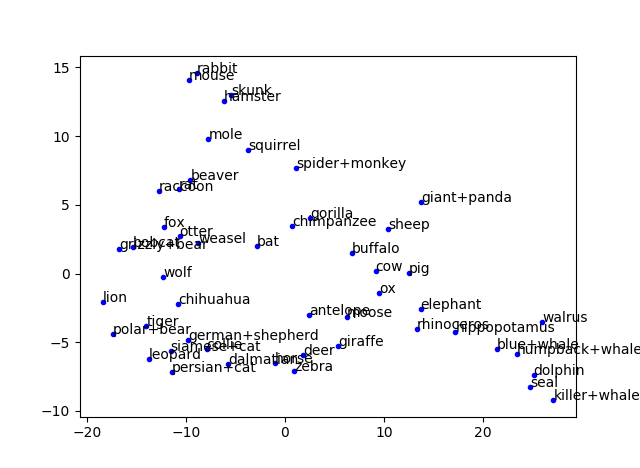
\includegraphics[width=48em]{q2_1.png}
    \caption{Question 2.1 ISOMAP}
    \label{fig:q2_1}
\end{figure}


\subsection{ISOMAP with Disconnected Graph}

\begin{figure}[h!]
    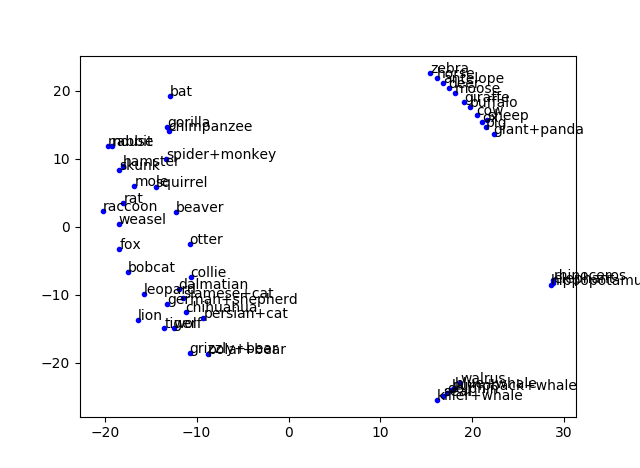
\includegraphics[width=48em]{q2_2.png}
    \caption{Question 2.2 ISOMAP with Disconnected Graph}
    \label{fig:q2_2}
\end{figure}

Code:
\begin{verbatim}

function ISOMAPdisconnectedGraph(X)
    k =2
    (n,d) = size(X)

    # Compute all distances
    D = distancesSquared(X,X)
    D = sqrt.(abs.(D))

    E = ones(n,n).*Inf

    for i in 1:n
        A = sortperm(D[i,:])
        for j in 2:k+1
          
          E[i,A[j]] =D[i,A[j]]
          E[A[j],i] =D[A[j],i]     
        end 
    end

    D = zeros(n,n)
    max = -Inf
    for i in 1:n
        for j in 1:n
         D[i,j] = dijkstra(E,i,j)
         if(D[i,j]!=Inf && D[i,j] > max)
            max =  D[i,j]
         end
        end
    end


    for i in 1:n
        for j in 1:n
             if(D[i,j]==Inf )
             D[i,j] = max
         end
        end
    end


    # Initialize low-dimensional representation with PCA
    model = PCA(X,2)
    Z = model.compress(X)
    

    funObj(z) = stress(z,D)

    Z[:] = findMin(funObj,Z[:])

    return Z
end

\end{verbatim}

\section{Neural Networks}

Various changes were made using combinations of the following items:
\items{
\item increasing $nHidden$ up to 150
\item increasing and decreasing the stochastic gradient step-size
\item increasing the number of stochastic iterations
\item adding momentum
\item adding L2 regularizer with various values for $\lambda$
\item using different activation functions, such as sigmoid, quadratic, $tanh + tanh^2$, composite of $tanh$ and quadratic
}

(standardization wasn't tried because the data we are graphing is 2D - i.e. we're only fitting 1 feature)

In the end, the best fit we found had the following parameters and added steps:
\items{
    \item $nHidden = 100$: deep neural network
    \item L2 regularizer with $\lambda = 0.01$: to reduce overfitting since we have so many layers
    \item momentum with same step-size: to improve optimization using stochastic gradient
    \item dynamic step size, going from $1e-4$ to $1e-7$: deep networks are sensitive to step-size, so the idea was to improve the performance of stochastic gradient by decreasing the step-size. We used decreasing step-sizes instead of using a constant small step-size to reduce runtime and the number of iterations required
    \item 50000 iterations: stochastic gradient with smaller step-sizes requires more iterations to reach optimal region
}

\begin{figure}[h!]
    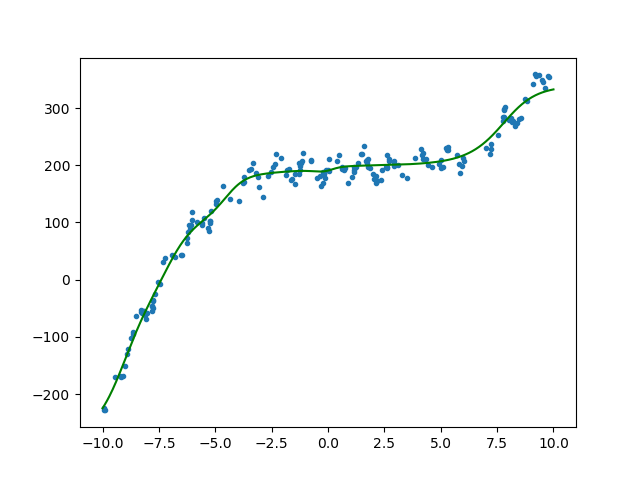
\includegraphics[width=48em]{a5_q3.png}
    \caption{Q5 Improved Neural Network Result}
    \label{fig:q3}
\end{figure}

\section{Very-Short Answer Questions}


\enum{
\item NMF is non-convex and can be minimized using projected gradient, where we run gradient descent on the loss function but set any negative values we get from gradient descent to zero.
\item A standard collaborative filtering model is trained, unsupervised, to minimize categorizing/clustering errors and is never trained to optimize the weights for prediction with supervised learning.
\item No. Both MDS and PCA can be viewed as some sort of compression algorithms, so there is always data loss, unless the data points in 3D all lie on the same 2D plane, but that's not guaranteed.
\item Euclidean distance is the length of the straight line drawn between two points, whereas geodesic distance is the length of the curve drawn between two points on a manifold. (i.e. Euclidean $\leq$ geodesic)
\item It results in a smooth loss that can be optimized with gradient descent and ensures the output of the perceptron is between 0 and 1 regardless of the domain of the input, so it can be used to represent probabilities
\item A deeper neural network likely has a higher test error but lower train error, while a neural network less deep likely has a high train error but lower test error.
\item 1) adding L2-regularizers for each layer of $W$ and optimizing the $\lambda$ of each regularizer, 2) early stopping (stops optimzation if validation error starts increasing), 3) dropout (setting some $x_i$ and $z_i$ in each layer to 0)
\item  Larger width results in smaller train error but larger test error, whereas smaller width results in larger train error but smaller test error.
}

\end{document}
